\section{Experiments and Evaluation}\label{sec:experiments}
% Describe our results based on different number of producer and consumer numbers.
% We implemented and evaluated our event processing architecture in Python and Java.

We have run multiple experiments to be able to select the right stream processing architecture for this task.
Our experiments include a set of experiments with varying numbers of event producers and consumer threads, as well as
other experiments with different numbers of threads and queue buffer sizes.

The main computation for Query 1 and Query 2 is a very small computation to get the last prices from a dictionary of stock symbols and then
compare the two values of $EMA_{38}$ and $EMA_{100}$ to identify breakouts. We have profiled our implementation and confirmed that the main implemented system
is an I/O bounded application, rather than a CPU bounded application, because of the quick computation for Query 1 and 2. The most time is
invested to get the data from the network (which is improved by having multiple producers), followed by organizing the stock price
dictionaries and iterating over the single events in an event batch.

By using vectorized bulk operations, we can avoid the linear time of iterating over the batch of events. This is implemented by using
vectorization within each of our multi-threaded consumers.

% Experiments with different number of event producer threads and consumer threads.
We have experimented with different numbers of producers and consumers.
Figure \ref{fig:evaluation} depicts Query 2 throughput results for different numbers of producers and consumers using small data batch of size 1k.
These results are produced by using the benchmark system provided by the DEBS 2022 Grand Challenge\footnote{\url{https://github.com/jawadtahir/CHALLENGER} last update June, 2022}.


\begin{figure}[]
    \begin{center}
        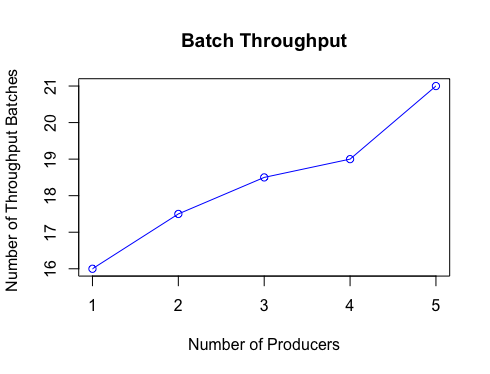
\includegraphics[width=0.5\textwidth]{./images/throughput.png}
        \caption{Query 2 throughput for different number of Producers. (Batch Size 1k)}
        \label{fig:evaluation}
    \end{center}
\end{figure}


%TODO!: Experiment with different architectures if we have any.

Our Java implementation can achieve higher performance because of some language features (Like static variable types and improved iterations over event batches).
According to the DEBS 2022 evaluation \cite{debs2022challenge} server, our Java implementation can achieve a latency of 19.99 seconds and a 88.21 batch per 
seconds with an event batch size of 10k (events arriving in batches of 10k).
